\section{Experimental Setup}
\label{section_5}
We conducted experiments for both the AXI bus-based and PCIe-based overlay accelerators.  
For the AXI bus-based system, the experimental software runs on the ARM processor of the Xilinx ZedBoard. 
For the PCIe-based accelerators (implemented using PCIe-Xillybus, RIFFA and DyRACT respectively), the experiments are run on an HP Z420 workstation (six 3.5 GHz Intel Xeon E5-1650 cores) with a Xilinx VC707 evaluation board plugged into the PCIe Gen2 slot of the motherboard. 

\subsection{AXI-Xillybus System}
The AXI-Xillybus system is using one 32-bit wide AXI ACP port for data transmission, running at a frequency of 100 MHz on the Xilinx ZedBoard. 
Hence the theoretical total bandwidth of this system is 800 MB/s, and the maximum streaming throughput is 400 MB/s in a full-duplex system. 

\subsubsection{AXI-Xillybus Loopback Test}
Before the accelerator system can be developed, we first ensure that the demonstration bundle provided by the Xillybus vendor operates correctly on our Zynq-based system. 
%The demonstration bundle includes an example FPGA design containing just a single FIFO used to loop the data back, along with a device driver and sample software code. 
We evaluate the performance of Xillybus by testing the round-trip data transmission throughput with the default settings, using sequential and parallel (multi-threading) programming for \textit{read} and \textit{write} functions respectively. 
%the write function and read function are executing sequentially by default, which means the read process has to wait until the write process has finished. 
%It is inefficient for a full-duplex interface to work in half-duplex mode, and so as to make full use of the Xillybus IP core, we adopt a multi-threading technique (using Pthreads) to improve its performance by creating two different threads for the write and read functions respectively. 

The bandwidth of the loopback test for AXI-Xillybus using different data block sizes is shown in Figure~\ref{axi_xillybus_loopback_bw}. 
As seen from this diagram, the single-threaded loopback test saturates at a throughput of around 150 MB/s (maximum of 160 MB/s) when the transfer size exceeds 8K words, while the multi-thread loopback test saturates (with a maximum throughput of 330 MB/s) when the transfer size exceeds 500K words. 
The two dashed lines indicate the theoretical throughput of the 32-bit AXI-ACP port running at 100 MHz.
The throughput of the multi-thread test surpasses that of the single-thread test for data block sizes exceeding 64K words, and for large block sizes achieves approximately twice the throughput. 
Creating Pthreads introduces a significant overhead for smaller transfer sizes, thus the multi-threading version is only applicable for large data transfers. 

\pgfplotsset{
	axis background/.style={fill=none},
	%tick style=mygrey2,
	%tick label style=mygrey2,
	grid=none,
	%xtick pos=left,
	%ytick pos=left,
	tick style={
		major grid style={style=white,line width=1pt},minor grid style=white,
%		major grid style={style=white,line width=1pt},minor grid style=mygrey3,
		%tick align=outside,
	},
	%minor tick num=4,
}

\begin{figure}[tb]
	\centering
	 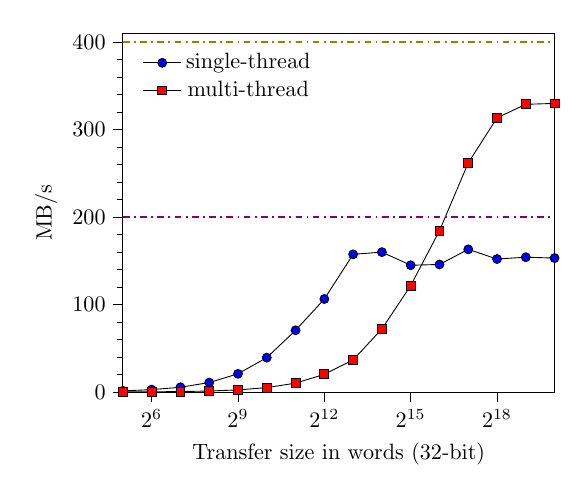
\begin{tikzpicture}[scale = 0.8]
	 \begin{axis}[
	 xmode=log,
	 log basis x={2},
	 xlabel=Transfer size in words (32-bit),
	 ymin=0,
	 ymax=410,
	 xmax = 1048576,
	 xmin = 32,
	 ylabel=MB/s,
%	 legend style={at={(0.3,0.8)},anchor=north}
	 legend pos=north west,
	 legend style={draw=none}
	 ]    

	\addplot [mark=*,mark options={fill=blue}] plot coordinates {
		(32,     1.4)
		(64,     2.8)
		(128,     5.5)
		(256,     10.9)
		(512,      20.9)
		(1024,     39.4)
		(2048,     70.6)
		(4096,     106.4)
		(8192,     157.5)
		(16384,    160.0)
		(32768,    145.0)
		(65536,    145.9)
		(131072,    163.2)
		(262144,    152.1)
		(524288,    154.2)
		(1048576,    153.2)	
	}; 
	 \addplot [mark=square*,mark options={fill=red}] plot coordinates {
	 	(32,     0.2)
	 	(64,     0.3)
	 	(128,     0.6)
	 	(256,     1.2)
	 	(512,     2.5)
	 	(1024,     5.1)
	 	(2048,     10.2)
	 	(4096,     20.3)
	 	(8192,      36.8)
	 	(16384,     72.2)
	 	(32768,    121.7)
	 	(65536,    184.5)
	 	(131072,    262)
	 	(262144,    313.5)
	 	(524288,    329)
	 	(1048576,    330)
	 }; 
	 \addplot [color=violet,thick,dash dot] plot coordinates {
	 	(32,     200)
		(64,     200)
		(128,     200)
		(256,     200)
		(512,     200)
		(1024,     200)
		(2048,     200)
		(4096,     200)
		(8192,     200)
		(16384,    200)
		(32768,    200)
		(65536,    200)
		(131072,    200)
		(262144,    200)
		(524288,    200)
		(1048576,   200)	
	 };

	 \addplot [color=olive,thick,dash dot] plot coordinates {
	(32,     400)
	(64,     400)
	(128,     400)
	(256,     400)
	(512,     400)
	(1024,     400)
	(2048,     400)
	(4096,     400)
	(8192,     400)
	(16384,    400)
	(32768,    400)
	(65536,    400)
	(131072,   400)
	(262144,   400)
	(524288,   400)
	(1048576,  400)	
};

	 \legend{single-thread\\multi-thread\\}
	 \end{axis}
	 \end{tikzpicture}	
	
	\caption[]{AXI-Xillybus loopback test evaluation.} 
	\label{axi_xillybus_loopback_bw}
	
\end{figure}


\subsubsection{AXI-Xillybus based Overlay Accelerator}
Xillybus provides an online IP core factory for users to customize the interface on demands.
%The accelerator and its data streams are shown in Figure~\ref{axi_xillybus_overlay}. 
In our design, two 32-bit streaming device files are instantiated for data acquisition and one 32-bit seekable device file is responsible for the instruction load and overlay setup. 
We evaluate the performance of the overlay accelerator which is an integration of the linear TM overlay as discussed in Section~\ref{section_3} and AXI-Xillybus interface, and compare to VectorBlox MXP~\cite{severance2013embedded}, in terms of bandwidth and area consumption. 
To perform this comparison, we use the set of kernels shown in Table~\ref{benchmarks_system}, which are extracted from compute intensive applications available from~\cite{gopalakrishnan2007finding, hoy2015performance}. 
Both the overlay accelerator and MXP are running on Xillinux-2.0, which is the latest Linux distribution released for ZedBoard (kernel 4.4), with AXI-Xillybus using the Pthread multi-threading technique with a data block transfer size of 1M words.

\begin{table}[tb]
	%	\renewcommand{\arraystretch}{1.2}
	\caption{DFG characteristics of benchmark set.}
	\label{benchmarks_system}
	\centering
	\resizebox{\columnwidth}{!}{
		\begin{tabular}{clccccc}
			\toprule
			\multirow{3}{*}{No.} & \multirow{3}{*}{Benchmark} &  \multicolumn{5}{c}{Characteristics}  \\ \cline{3-7}
			&                            &  I/O  & graph &  op   & graph & graph \\
			&                            & nodes & edges & nodes & depth & width \\ \midrule
			1.          & chebyshev                  &  1/1  &  12   &   7   &   7   &   1   \\
			2.          & mibench                    &  3/1  &  22   &  13   &   6   &   3   \\
			3.          & qspline                    &  7/1  &  50   &  25   &   8   &   6   \\
			4.          & fft                        &  6/4  &  24   &  10   &   3   &   4   \\
			5.          & kmeans                     & 16/1  &  39   &  23   &   5   &   8   \\
			6.          & mm                         & 16/1  &  31   &  15   &   4   &   8   \\
			7.          & spmv                       & 16/2  &  30   &  14   &   4   &   8   \\
			8.          & stencil                    & 15/2  &  30   &  14   &   5   &   6   \\ \bottomrule
		\end{tabular}
	}
\end{table}

Figure~\ref{axi_xillybus_mxp_bw} shows the performance of a single 32-bit linear TM overlay (AXI-Xillybus-Overlay) and a 16-lane 32-bit MXP (MXP-V16) implemented on a ZedBoard for the benchmarks given in Table~\ref{benchmarks_system}. 
As seen from the figure, MXP-V16 outperforms AXI-Xillybus-Overlay over all benchmarks (with the exception of `chebyshev'). 
Table~\ref{xillybus_mxp_area} shows the hardware resource usage of the AXI-Xillybus based overlay accelerator and MXP-V16. 
As seen from this table, AXI-Xillybus-Overlay is much more area efficient, and consumes only 19.8\% LUTs, 26.1\% FFs, 7.6\% BRAMs and 7.1\% DSP blocks, compared to MXP-V16. 

\pgfplotsset{
	axis background/.style={fill=white},
	tick style=black,
	tick label style=black,
	grid=both,
	xtick pos=left,
	ytick pos=left,
	tick style={
		major grid style={style=white,line width=1pt},minor grid style=white,
		tick align=outside,
	},
	minor tick num=4,
}

\begin{figure}[tb]
	\centering
	\pgfplotstableread{
		0		379.7	342		217		195.4
		1		245.7	317		226.7	292.6
		2		203.1	422		227.5	472.6
		3		94		158.7	225.6	380.9
		4		83.9	207.9	233.5	578.5
		5		53.9	142		229.9	605.9
		6		49.7	127.9	227.1	584.7
		7		52.7	134		225.8	574.3
	}\datathroughput	
%	\pgfplotstableread{
%		0		379.7	342		434		390
%		1		237		317		292		390
%		2		191.4	422		245		540
%		3		94		158.7	376		635
%		4		77.8	207.9	230		942
%		5		51.4	142		233		644
%		6		47.2	127.9	243		658
%		7		50.6	134		246		651
%	}\datathroughput
	\subfigure[Data processing throughput in MB/s]{
		\begin{tikzpicture}[scale = 0.9]
		\centering
		\begin{axis}[
%		axis y line=left,
		ybar=0pt,
		width=17cm,
		x = 0.85cm,
		height=5.3cm,
		ymin=0,
		ymax=1000,        
		ylabel={MB/s},
		grid style={dotted,gray},
		ymajorgrids=true,
		%	nodes near coords,    
		xtick=data,
		bar width = 5, %0.2
		xticklabels = {
			\strut chebyshev,
			\strut mibench,
			\strut qspline,
			\strut fft,
			\strut kmeans,
			\strut mm,
			\strut spmv,
			\strut stencil                                     
		},
		x tick label style={rotate=45, anchor=north east, inner sep=0mm},
		major x tick style = {opacity=0},
		minor x tick num = 1,
		minor tick length=1ex,
		%	every node near coord/.append style={
		%		anchor=west,
		%		rotate=90,
		%		font=\tiny
		%	},
		]
		
		\addplot[draw=black,fill=blue, draw opacity=1] table[x index=0,y index=3] \datathroughput;\label{MB_xillybus_axi}
		\addplot[draw=black,fill=red, draw opacity=1] table[x index=0,y index=4]   \datathroughput;\label{MB_mxp} 					
		\end{axis}
		
		\node [draw=none, fill=white] at (rel axis cs: 0.4, 0.8) {\shortstack[l]{
				\ref{MB_xillybus_axi} AXI-Xillybus-Overlay \\ \ref{MB_mxp} MXP-V16 }};	
		\end{tikzpicture}
	}

	\subfigure[Throughput in MOPS]{
		\begin{tikzpicture}[scale = 0.9]
		\centering
		\begin{axis}[
%		axis y line=right,
		ybar=0pt,
		width=17cm,
		x = 0.85cm,
		height=5.3cm,
		ymin=0,
		ymax=800,        
		ylabel={MOPS},
		grid style={dotted,gray},
		ymajorgrids=true,
		%	nodes near coords,    
		xtick=data,
		bar width = 5, %0.2
		xticklabels = {
			\strut chebyshev,
			\strut mibench,
			\strut qspline,
			\strut fft,
			\strut kmeans,
			\strut mm,
			\strut spmv,
			\strut stencil                                   
		},
		x tick label style={rotate=45, anchor=north east, inner sep=0mm},
		major x tick style = {opacity=0},
		minor x tick num = 1,
		minor tick length=1ex,
		%	every node near coord/.append style={
		%		anchor=west,
		%		rotate=90,
		%		font=\tiny
		%	},
		]
		
		\addplot[draw=black,fill=blue, draw opacity=1] table[x index=0,y index=1] \datathroughput;\label{MOPS_xillybus_axi}
		\addplot[draw=black,fill=red, draw opacity=1] table[x index=0,y index=2]   \datathroughput;\label{MOPS_mxp} 					
		\end{axis}
		
		\node [draw=none, fill=white] at (rel axis cs: 0.4, 0.8) {\shortstack[l]{
				\ref{MOPS_xillybus_axi} AXI-Xillybus-Overlay \\ \ref{MOPS_mxp} MXP-V16 }};	
		\end{tikzpicture}
	}
	
	\caption{Performance comparison for the benchmarks using a transfer size of 1M words.}
	\label{axi_xillybus_mxp_bw}
\end{figure}

The MXP memory system is based on one 64-bit AXI HP port running at a frequency of 110 MHz while AXI-Xillybus is based on a single 32-bit AXI ACP port running at a frequency of 100 MHz. 
This corresponds to a theoretical maximum throughput of 880 MB/s for MXP-V16 and 400 MB/s for AXI-Xillybus-Overlay. 
As seen from Figure~\ref{axi_xillybus_mxp_bw}, MXP-V16 achieves a throughput of 460.6 MB/s (52.3\% of theoretical maximum) on average while AXI-Xillybus has a throughput of 226.6 MB/s (56.6\% of theoretical maximum) on average. 
%Figure~\ref{axi_xillybus_mxp_bw} indicates that AXI-Xillybus-V3 has a worse performance for the benchmarks with a larger number of I/O nodes. 
The throughput of AXI-Xillybus is about half of that of MXP-V16, mainly due to AXI-Xillybus using only 32-bit of the available 64-bit ACP port while MXP-V16 uses the full 64-bit HP port. 


\begin{table}[tb]
	%	\renewcommand{\arraystretch}{1.2}
	\caption{Area overhead of AXI bus-based systems.}
	\label{xillybus_mxp_area}
	\centering
	\resizebox{\columnwidth}{!}{
		\begin{tabular}{lrrrr}
			\toprule
			\multirow{2}{*}{System} &                \multicolumn{4}{c}{Resource Usage}                \\ \cline{2-5}
			&            LUTs &              FFs &        BRAMs &         DSPs \\ \midrule
			Overlay                 &           1,747 &            1,954 &            0 &            8 \\
			AXI-Xillybus            &           4,000 &            3,844 &            5 &            0 \\ \midrule
			MXP-V16                 &          28,974 &           22,174 &           66 &          112 \\ \midrule
			\textbf{Available}      & \textbf{53,200} & \textbf{106,400} & \textbf{140} & \textbf{220} \\ \bottomrule
		\end{tabular}
	}
\end{table}

Although the AXI bus-based Xillybus provides an area efficient interface solution for the Xilinx Zynq SoC, the throughput is still far below the theoretical maximum shown in Table~\ref{theo_bw}. 
This is mainly due to not making good use of the available HP/ACP ports (Xillybus uses only one 32-bit port which is operating at a frequency of 66.7\% of the theoretical maximum that the AXI bus on Zynq can support). 


\subsection{PCIe System}
Our PCIe system is based on the Gen2$\times$8 PCIe interface running at a frequency of 250 MHz on the Xilinx VC707 platform, which corresponds to a maximum bandwidth of 8000 MB/s and hence a maximum streaming throughput of 4000 MB/s for a full-duplex system. 


\subsubsection{Loopback Test}
%%% Combine Xillybus, RIFFA and DyRACT together %%%
Similar to the AXI-Xillybus System, we first evaluate the baseline performance of the three PCIe interfaces using a loopback test. 

\noindent \textbf{PCIe-Xillybus}
Xillybus has been upgraded to a new version (PCIe-Xillybus) to support high performance PCIe interface communication since 2015. 
The block diagram of PCIe-Xillybus for data loopback is almost the same as that of AXI-Xillybus, except that the 32-bit FIFO is replaced with a 128-bit FIFO and the Xillybus hardware module \textit{Xillybus.v} (including the Xillybus IP core and a Xilinx 7 series integrated block for PCIe) is connected to an HP Z420 workstation via the PCIe link. 
Similar to AXI-Xillybus, we developed two host programs to evaluate the round-trip bandwidth in both half-duplex and full-duplex mode. 

\noindent \textbf{RIFFA}
The loopback test design of RIFFA framework is slightly different from that of Xillybus. 
A first word fall through (FWFT) FIFO is used for data transmission between the RIFFA IP core and the user logic applications. 
Data transmission is under the control of a finite state machine (FSM), which executes the upstream transfers and downstream transfers in different processing states.  
Thus, it is not possible to achieve full-duplex data transmission. 

\noindent \textbf{DyRACT}
\todo[inline]{Add a description of DyRACT loopback design}


The bandwidth of the loopback test for PCIe-Xillybus, RIFFA and DyRACT using different data block sizes is shown in Figure~\ref{pcie_xillybus_riffa_loopback_bw}. 
The two dashed lines indicate the theoretical bandwidth of the Gen2$\times$8 PCIe interface running at 250 MHz.

%\pgfdeclarelayer{background}
%\pgfdeclarelayer{foreground}
%\pgfsetlayers{background,main,foreground}

\pgfplotsset{
	axis background/.style={fill=none},
	%tick style=mygrey2,
	%tick label style=mygrey2,
	grid=none,
	%xtick pos=left,
	%ytick pos=left,
	tick style={
		major grid style={style=white,line width=1pt},minor grid style=white,
%		major grid style={style=white,line width=1pt},minor grid style=mygrey3,
		%tick align=outside,
	},
	%minor tick num=4,
}

\begin{figure}[tb]
	\centering
	 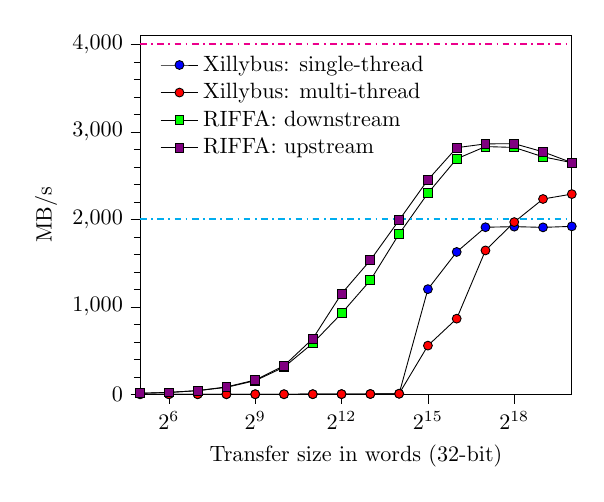
\begin{tikzpicture}[scale = 0.8]
	 \begin{axis}[
	 xmode=log,
	 log basis x={2},
	 xlabel=Transfer size in words (32-bit),
	 ymin=0,
	 ymax=4100,
	 xmax = 1048576,
	 xmin = 32,
	 ylabel=MB/s,
%	 legend style={at={(0.3,0.8)},anchor=north}
	 legend cell align={left},
	 legend pos=north west,
	 legend style={draw=none}
	 ]    

	\addplot [mark=*,mark options={fill=blue}] plot coordinates {
		(32,     0)
		(64,     0)
		(128,    0.05)
		(256,     0.1)
		(512,      0.2)
		(1024,     0.35)
		(2048,     0.7)
		(4096,     1.45)
		(8192,     2.9)
		(16384,    5.85)
		(32768,    1201.5)
		(65536,    1626.5)
		(131072,   1909.1)
		(262144,   1915.8)
		(524288,   1907.7)
		(1048576,  1919.1)	
	}; 
	 \addplot [mark=*,mark options={fill=red}] plot coordinates {
	 	(32,     0)
	 	(64,     0)
	 	(128,    0.04)
	 	(256,    0.08)
	 	(512,    0.16)
	 	(1024,   0.32)
	 	(2048,   0.68)
	 	(4096,   1.36)
	 	(8192,   2.76)
	 	(16384,  5.85)
	 	(32768,  556)
	 	(65536,  864)
	 	(131072, 1644)
	 	(262144, 1968)
	 	(524288, 2232)
	 	(1048576, 2288)
	 }; 
	 
	 \addplot [mark=square*,mark options={fill=green}] plot coordinates {
	 	(32,     11.1)
	 	(64,     20.3)
	 	(128,    41.0)
	 	(256,    78.8)
	 	(512,    155.0)
	 	(1024,   310.0)
	 	(2048,   583.0)
	 	(4096,   924.6)
	 	(8192,   1302.1)
	 	(16384,  1832.8)
	 	(32768,  2297.8)
	 	(65536,  2691.1)
	 	(131072, 2831.3)
	 	(262144, 2821.2)
	 	(524288, 2713.9)
	 	(1048576,2647.7)	
	 }; 
	 \addplot [mark=square*,mark options={fill=violet}] plot coordinates {
	 	(32,     11.1)
	 	(64,     21.0)
	 	(128,    41.4)
	 	(256,    83.5)
	 	(512,    162.8)
	 	(1024,   325.5)
	 	(2048,   635.2)
	 	(4096,   1148.9)
	 	(8192,   1531.9)
	 	(16384,  1990.4)
	 	(32768,  2451.0)
	 	(65536,  2818.5)
	 	(131072, 2862.0)
	 	(262144, 2864.5)
	 	(524288, 2771.1)
	 	(1048576,2647.7)
	 }; 
	 
	 \addplot [color=cyan,thick,dash dot] plot coordinates {
	 	(32,     2000)
		(64,     2000)
		(128,     2000)
		(256,     2000)
		(512,     2000)
		(1024,     2000)
		(2048,     2000)
		(4096,     2000)
		(8192,     2000)
		(16384,    2000)
		(32768,    2000)
		(65536,    2000)
		(131072,    2000)
		(262144,    2000)
		(524288,    2000)
		(1048576,   2000)	
	 };

	 \addplot [color=magenta,thick,dash dot] plot coordinates {
		(32,     4000)
		(64,     4000)
		(128,     4000)
		(256,     4000)
		(512,     4000)
		(1024,     4000)
		(2048,     4000)
		(4096,     4000)
		(8192,     4000)
		(16384,    4000)
		(32768,    4000)
		(65536,    4000)
		(131072,   4000)
		(262144,   4000)
		(524288,   4000)
		(1048576,  4000)	
};
	
	\legend{Xillybus: single-thread\\Xillybus: multi-thread\\RIFFA: downstream\\RIFFA: upstream\\}
	\end{axis}
	\end{tikzpicture} 
%	\label{riffa_loopback_bw}
%	}
	
	\caption[]{PCIe system loopback test evaluation.} 
	\label{pcie_xillybus_riffa_loopback_bw}
	
\end{figure}


For PCIe-Xillybus system, the data transmission is very slow when the transfer size is less than 32K words. 
This is due to large system overhead for a data buffer size of less than 128 KBytes~\cite{xillybus2018}. 
The single-threaded loopback test saturates at a throughput of 1900 MB/s when the transfer size exceeds 128K words, while the multi-thread loopback test saturates (with a maximum throughput of 2300 MB/s) when the transfer size exceeds 500K words. 
The throughput of the multi-thread test surpasses that of the single-thread test for data block sizes exceeding 256K words, and achieves around 1.2$\times$ higher bandwidth when transferring 1M words. 
Although the throughput of the multi-thread test is not as expected (twice that of the single-thread test), it shows better performance for the transmission of large data blocks. 


For RIFFA system, both the upstream transfers (read) and downstream transfers (write) saturate at around 2.85 GB/s when the transfer size is equal to 128K sample words, corresponding a total bandwidth of 2.85 GB/s, as read and write cannot happen simultaneously. 
The bandwidth degrades slightly when the transfer size exceeds 128k words due to the overutilization of BRAMs.
As mentioned previously, the RIFFA hardware was not developed for full-duplex data transmission. 
Hence the send and receive functions will execute sequentially and it is useless to use multi-threading techniques as was done for Xillybus. 


For DyRACT system,  \todo[inline]{Analysis of DyRACT loopback test performance}


\subsubsection{PCIe-based Overlay Accelerator}
In the PCIe-based overlay accelerator framework, we propose replicating four 32-bit linear TM overlays, interfacing with two 128-bit FIFOs to make full use of the data width.
The overlay interfacing with PCIe-Xillybus or RIFFA has to hardcode the instructions to the FUs as it has no access to the FPGA RAMs directly. 
Thus reconfiguring the overlay is inevitable when the application kernel changes. 
In comparison, the overlay interfacing with DyRACT is able to customise three memory arrays to restore the instructions along with their tags to the FUs, and the number of input data or the value of II minus one (II-1). 


Figure~\ref{pcie_xillybus_riffa_bw} shows the performance of four 32-bit linear TM overlays integrated with PCIe-Xillybus (PCIe-Xillybus-Overlay), RIFFA (RIFFA-Overlay) and DyRACT (DyRACT-Overlay), respectively. 
PCIe-Xillybus-Overlay uses a block size of 1M words with the Pthread multi-threading technique, while RIFFA-Overlay and DyRACT-Overlay use a block size of 128K words. 
All these overlay accelerators are running on an Ubuntu 14.04.5 workstation (six 3.5 GHz Intel Xeon E5-1650 cores) with a Xilinx VC707 evaluation board plugged into the PCIe Gen2 slot of the motherboard. 
As can be seen from Figure~\ref{pcie_xillybus_riffa_bw}, DyRACT-Overlay achieves an average throughput of 1540 MB/s (38.5\% of theoretical maximum), which is around 18\% higher than RIFFA-Overlay with an average throughput of 1300 MB/s and 4.3$\times$ better than PCIe-Xillybus-Overlay with an average throughput of 358 MB/s (9\% of theoretical maximum). 
The ratio of the throughput in Mega-operations per second (MOPS) is proportional to that of data processing throughput in MB/s. 
DyRACT-Overlay proves to be the best accelerator in terms of throughput. 
%\todo[inline]{Add some in-depth analysis for the overlay accelerators}
Although all the three implementations show slight fluctuation of the throughput in MB/s, it has dramastic changes in terms of MOPS. 
This is mainly due to the large number of I/O ports (especially for the last four benchmarks), which corresponds to larger II values. 
In a nutshell, the linear TM overlay accelerators are more suitable to the benchmarks with less number of I/O ports. 

\pgfplotsset{
	axis background/.style={fill=white},
	tick style=black,
	tick label style=black,
	grid=both,
	xtick pos=left,
	ytick pos=left,
	tick style={
		major grid style={style=white,line width=1pt},minor grid style=white,
		tick align=outside,
	},
	minor tick num=4,
	compat = 1.3,
}

\begin{figure}[tb]
	\centering
	\pgfplotstableread{
		0		677		1448	2081	386.9		828		 1190
		1		381		1469	1680	351.5		1355	 1550
		2		312		1250	1657	349.5		1400	 1856
		3		155		582		683		372			1396	 1640
		4		127		494		578		353.4		1375	 1610
		5		83		321		324		354			1369	 1383
		6		76		300		328		347.3		1370	 1496
		7		82		310		370		351.3		1328	 1587
	}\datathroughput	
	\subfigure[Data processing throughput in MB/s]{
		\begin{tikzpicture}[scale = 0.9]
		\centering
		\begin{axis}[
%		axis y line=left,
		ybar=0pt,
		width=17cm,
		x = 0.85cm,
		height=5.3cm,
		ymin=0,
		ymax=3000,        
		ylabel={MB/s},
		grid style={dotted,gray},
		ymajorgrids=true,
		%	nodes near coords,    
		xtick=data,
		bar width = 5, %0.15
		xticklabels = {
			\strut chebyshev,
			\strut mibench,
			\strut qspline,
			\strut fft,
			\strut kmeans,
			\strut mm,
			\strut spmv,
			\strut stencil                                     
		},
		x tick label style={rotate=45, anchor=north east, inner sep=0mm},
		major x tick style = {opacity=0},
		minor x tick num = 1,
		minor tick length=1ex,
		%	every node near coord/.append style={
		%		anchor=west,
		%		rotate=90,
		%		font=\tiny
		%	},
		]
		
		\addplot[draw=black,fill=blue, draw opacity=1] table[x index=0,y index=4] \datathroughput;\label{MB_xillybus_pcie}
		\addplot[draw=black,fill=red, draw opacity=1] table[x index=0,y index=5]   \datathroughput;\label{MB_riffa} 
		\addplot[draw=black,fill=green, draw opacity=1] table[x index=0,y index=6]   \datathroughput;\label{MB_dyract} 						
		\end{axis}
		
		\node [draw=none, fill=white, font=\small] at (rel axis cs: 0.6, 0.8) {\shortstack[l]{
				\ref{MB_xillybus_pcie} PCIe-Xillybus-Overlay  \ref{MB_riffa} RIFFA-Overlay \\ \ref{MB_dyract} DyRACT-Overlay }};	
		\end{tikzpicture}
	}

	\subfigure[Throughput in MOPS]{
		\begin{tikzpicture}[scale = 0.9]
		\centering
		\begin{axis}[
%		axis y line=right,
		ybar=0pt,
		width=17cm,
		x = 0.85cm,
		height=5.3cm,
		ymin=0,
		ymax=3300,        
		ylabel={MOPS},
		grid style={dotted,gray},
		ymajorgrids=true,
		%	nodes near coords,    
		xtick=data,
		bar width = 5, %0.15
		xticklabels = {
			\strut chebyshev,
			\strut mibench,
			\strut qspline,
			\strut fft,
			\strut kmeans,
			\strut mm,
			\strut spmv,
			\strut stencil                                      
		},
		x tick label style={rotate=45, anchor=north east, inner sep=0mm},
		major x tick style = {opacity=0},
		minor x tick num = 1,
		minor tick length=1ex,
		%	every node near coord/.append style={
		%		anchor=west,
		%		rotate=90,
		%		font=\tiny
		%	},
		]
		
		\addplot[draw=black,fill=blue, draw opacity=1] table[x index=0,y index=1] \datathroughput;\label{MOPS_xillybus_pcie}
		\addplot[draw=black,fill=red, draw opacity=1] table[x index=0,y index=2]   \datathroughput;\label{MOPS_riffa} 	
		\addplot[draw=black,fill=green, draw opacity=1] table[x index=0,y index=3]   \datathroughput;\label{MOPS_dyract} 					
		\end{axis}
		
		\node [draw=none, fill=white, font=\small] at (rel axis cs: 0.6, 0.8) {\shortstack[l]{
				\ref{MOPS_xillybus_pcie} PCIe-Xillybus-Overlay  \ref{MOPS_riffa} RIFFA-Overlay \\ \ref{MOPS_dyract} DyRACT-Overlay }};	
		\end{tikzpicture}
	}
	
	\caption{Performance comparison for the benchmarks.}
	\label{pcie_xillybus_riffa_bw}
\end{figure}

Table~\ref{pcie_xillybus_riffa_area} shows a breakdown of the FPGA resource usage of the overlay, PCIe-Xillybus, RIFFA and DyRACT. 
%RIFFA-Overlay consumes 15\% fewer LUTs, 49\% more FFs, 29$\times$ more BRAMs and the same DSP blocks compared to PCIe-Xillybus-Overlay. 
PCIe-Xillybus-Overlay consumes least number of FFs (33\% fewer than RIFFA-Overlay), while RIFFA-Overlay costs least number of LUTs (21\% fewer than DyRACT-Overlay) and DyRACT-Overlay is most area efficient in BRAMs consumption (96\% fewer than RIFFA-Overlay). 
While the logic and DSP resources used are comparable among all these implementations, there is a big difference in the BRAM utilization specifically for RIFFA-Overlay.
This is due to the half-duplex mode of the RIFFA interface, resulting in a significant BRAM consumption to implement the two large depth FWFT FIFOs. 
Developing a full-duplex RIFFA based system would minimize the BRAM resource usage. 
At current stage, DyRACT-Overlay and PCIe-Xillybus-Overlay are much better than RIFFA-Overlay in terms of area efficiency. 

\begin{table}[tb]
	%	\renewcommand{\arraystretch}{1.2}
	\caption{Area overhead of PCIe-based systems.}
	\label{pcie_xillybus_riffa_area}
	\centering
	\resizebox{\columnwidth}{!}{
		\begin{tabular}{lrrrr}
			\toprule
			\multirow{2}{*}{System} &                  \multicolumn{4}{c}{Resource Usage}                   \\ \cline{2-5}
			&             LUTs &              FFs &          BRAMs &           DSPs \\ \midrule
			Overlay                 &            6,988 &            7,816 &              0 &             32 \\
			PCIe-Xillybus           &            9,039 &            4,672 &           14.5 &              0 \\
			RIFFA                   &            6,669 &           10,765 &          289.5 &              0 \\
			DyRACT                  &           10,356 &            8,648 &             10 &              0 \\
			\textbf{Available}      & \textbf{303,600} & \textbf{607,200} & \textbf{1,030} & \textbf{2,800} \\ \bottomrule
		\end{tabular}
	}
\end{table}
